\Chapter{Játék működése felhasználói szemszögből}

\Section{Bejelentkezés}

\begin{figure}[h!]
\centering
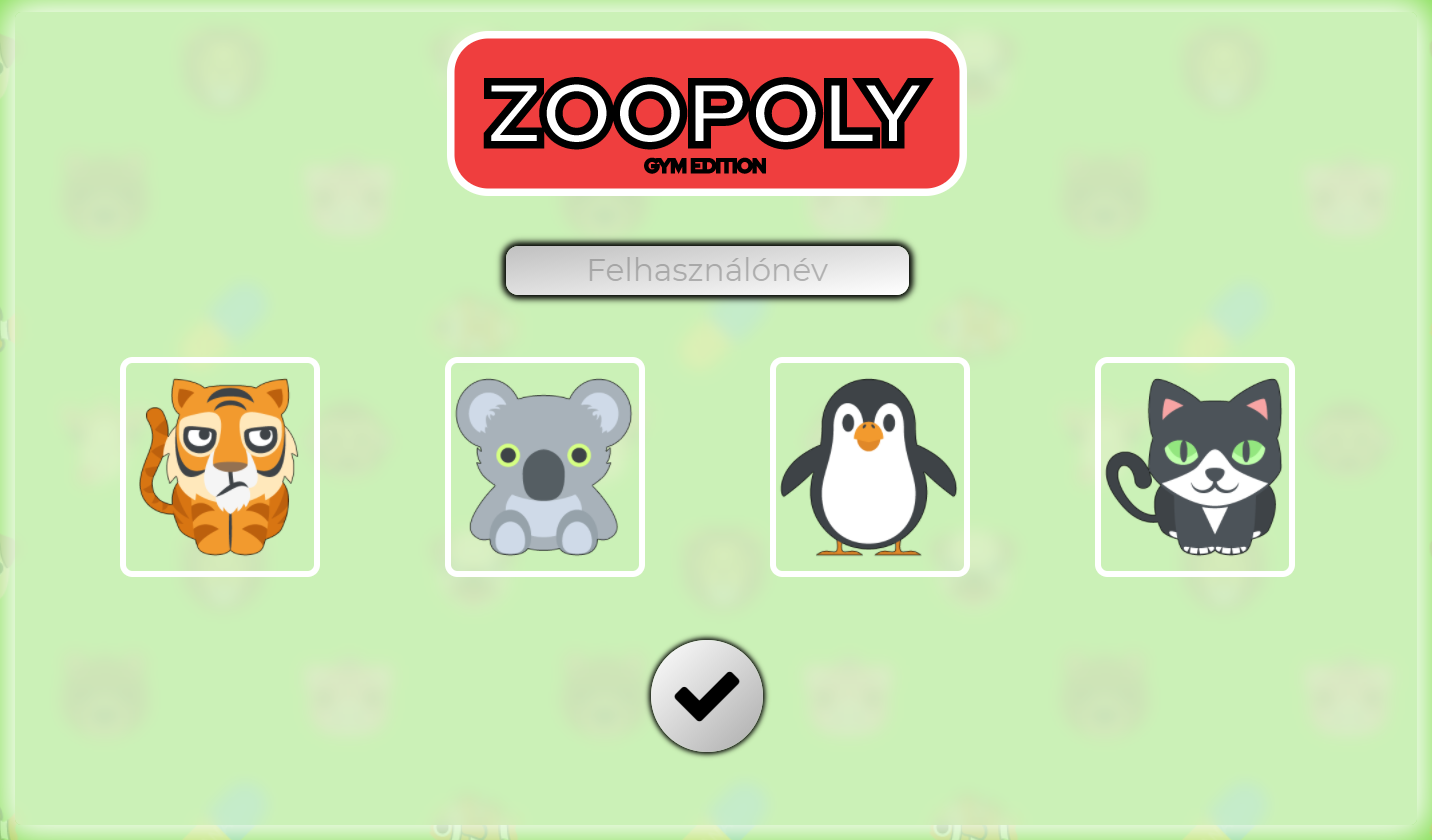
\includegraphics[width=\textwidth]{images/a5187162fb81495697aab2f5f49d6bd0.png}
\caption{Bejelentkezési felület}
\label{fig:ff}
\end{figure}

A felhasználónak meg kell adnia egy felhasználónevet, illetve választania kell egy kinézetet, amivel játszani szeretne. Fontos kikötés, hogy olyan felhasználónevet válasszon, amelyet még egyik játékos sem választott, és köteles egy tetszőleges kinézetet is választania. Ezután a pipára kattintva egy várakozó szobába lesz irányítva.

\Section{Várakozó szoba}

Az első bejelentkezett játékos megkapja az úgynevezett host jelzőt, ami jogot ad neki, hogy használja a parancsokat a Chat felületen. A használható parancsokat listázva találja meg.

Parancsok:
\begin{itemize}
	\item /start - Játék indítása
	\item /clear - Üzenetek eltüntetése
	\item /alog - Log aktiválása
	\item /dlog - Log deaktiválása
\end{itemize}
Ezen a felületen csupán annyi dolga van a nem host játékosnak, hogy megvárja amíg a host titulussal rendelkező játékos elindítsa a játékot.

\Section{Chat}

\begin{figure}[h!]
\centering
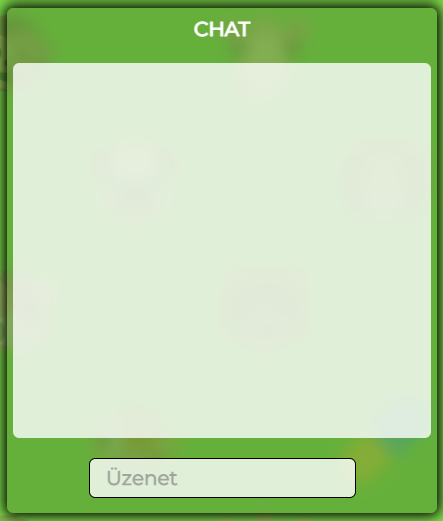
\includegraphics[scale=0.4]{images/50363fc646a02ca3f5dd4684b7066bac.png}
\caption{Chat felület}
\label{fig:ff}
\end{figure}

Mindenkinek lehetősége van üzenetet írni mások számára. Ezt úgy teheti meg, hogy az Üzenet mezőbe begépeli a kívánt szöveget, majd az Enter lenyomásával elküldi. Parancsok beírására csak a host-nak van lehetősége, ezek nem jelennek meg a többi játékos számára. A “Szerencsekártya” mezőre lépve a játék folyamán itt jelenik meg a kártya szövege.
\newpage
\Section{Játék kezdete}

\begin{figure}[h!]
\centering
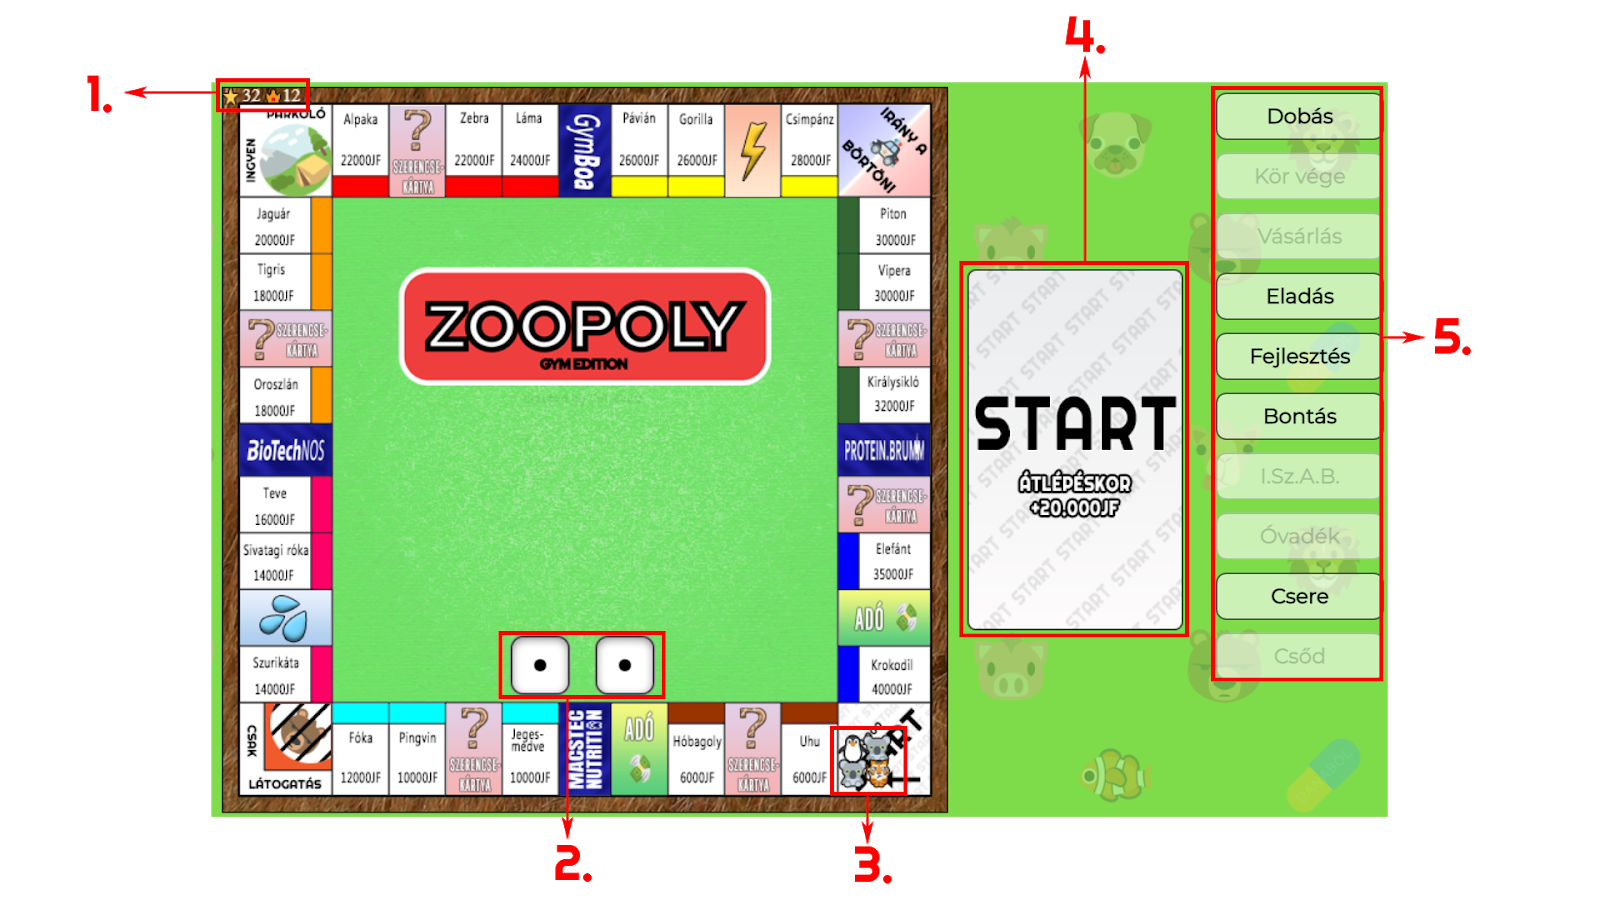
\includegraphics[scale=0.25]{images/Nevtelen-3.png}
\caption{Játéktábla}
\label{fig:ff}
\end{figure}
Megjelenik maga a játéktábla és a játékos által használható gombok.
\begin{enumerate}
	\item A játékon belül jelenleg ennyi szabadon felhasználható Csillag illetve Korona van még.
	\item A játékos által dobott számokat ezeken a dobókockákon látni.
	\item A játékosok bábúi amivel lépnek a táblán.
	\item Az aktuális mező kártyája, ami dobás után változik.
	\item A játékos által használható gombok. Az elszürkült gombok jelenleg nem használhatóak a játékos számára.
\end{enumerate}

\Section{Gombok}

Ebben az alfejezetben bemutatom a játékosok számára használható gombokat, illetve azok funkcióit.

\begin{itemize}
	\item Dobás - A játékos dob a dobókockákkal.
	\item Kör vége - A játékos befejezi a körét, a következő játékos lesz soron.
	\item Vásárlás - Ha a játékos a körben már használta a dobókockákat, és olyan mezőre lép ami még megvásárolható, megvásárolja azt.
	\item Eladás - Megvásárolt telek eladása a bank számára.
	\item Fejlesztés - Megvásárolt telek fejlesztése.
	\item Bontás - Megvásárolt telek visszafejlesztése.
	\item I.Sz.A.B. - “Ingyen Szabadulhatsz A Börtönből” kártya felhasználása, csak akkor használható ha a játékos börtönben van.
	\item Óvadék - 5.000JF óvadék kifizetése, csak akkor használható ha a játékos börtönben van.
	\item Csere - Kereskedhet egy általa kiválasztott játékossal.
	\item Csőd - Amennyiben a játékos nem tudja kifizetni a tartozását, csődöt tud mondani, ez a játék végét jelenti számára. Csak akkor használható, ha tartozással rendelkezik.
\end{itemize}

\Section{Online Játékosok fül, inventory megjelenítése}

\begin{figure}[h!]
\centering
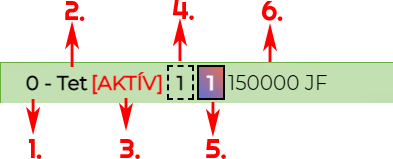
\includegraphics[scale=0.6]{images/Nevtelen-7.png}
\caption{Játékossal kapcsolatos információk}
\label{fig:ff}
\end{figure}

Az Online Játékosok ablakban megjelennek a játékosok adatai.
\begin{enumerate}
	\item Mező, amelyen a játékos jelenleg tartózkodik.
	\item Játékos neve
	\item Ha aktív a játékos, megjelenik az AKTÍV felirat.
	\item Ennyi ideig tartózkodik a játékos a börtönben.
	\item Ennyi “Ingyen Szabadulhatsz A Börtönből” kártyával rendelkezik a játékos.
	\item Ennyi összeggel rendelkezik a játékos.
\end{enumerate}
\newpage
Egy játékos fülre kattintva pedig megjelenik, hogy milyen monopóliumokkal rendelkezik. Az ablak tetején a választott játékos neve található.

\begin{figure}[h!]
\centering
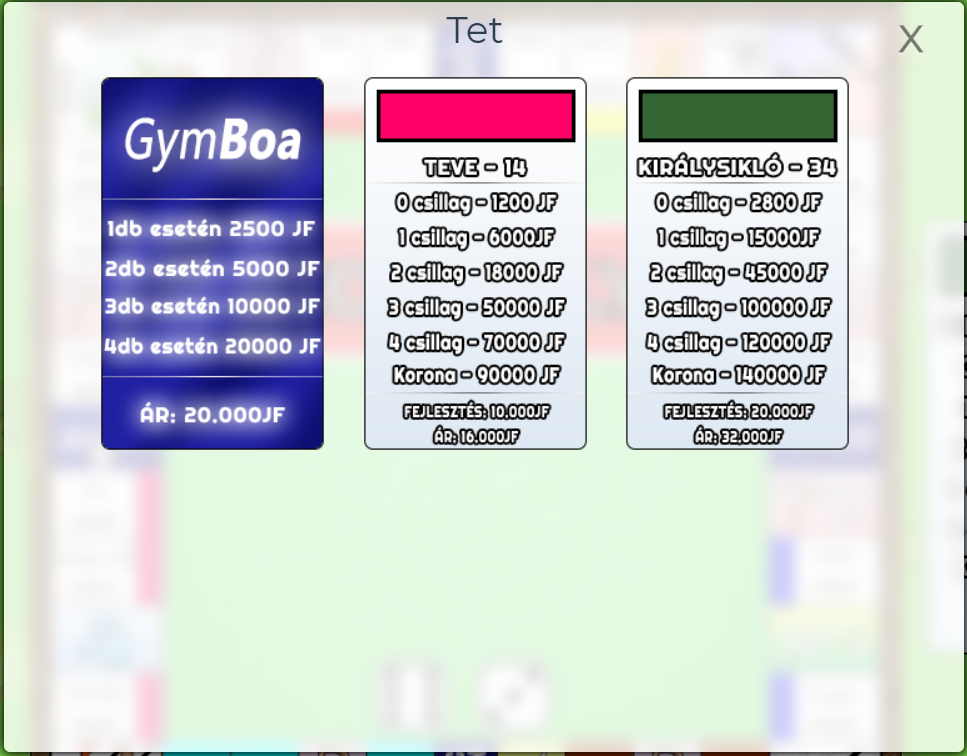
\includegraphics[scale=0.4]{images/ca07dc6cdaa3b06f2ed463e12650af68.png}
\caption{Inventory megjelenítése}
\label{fig:ff}
\end{figure}

\Section{Játék vége}

\begin{figure}[h!]
\centering
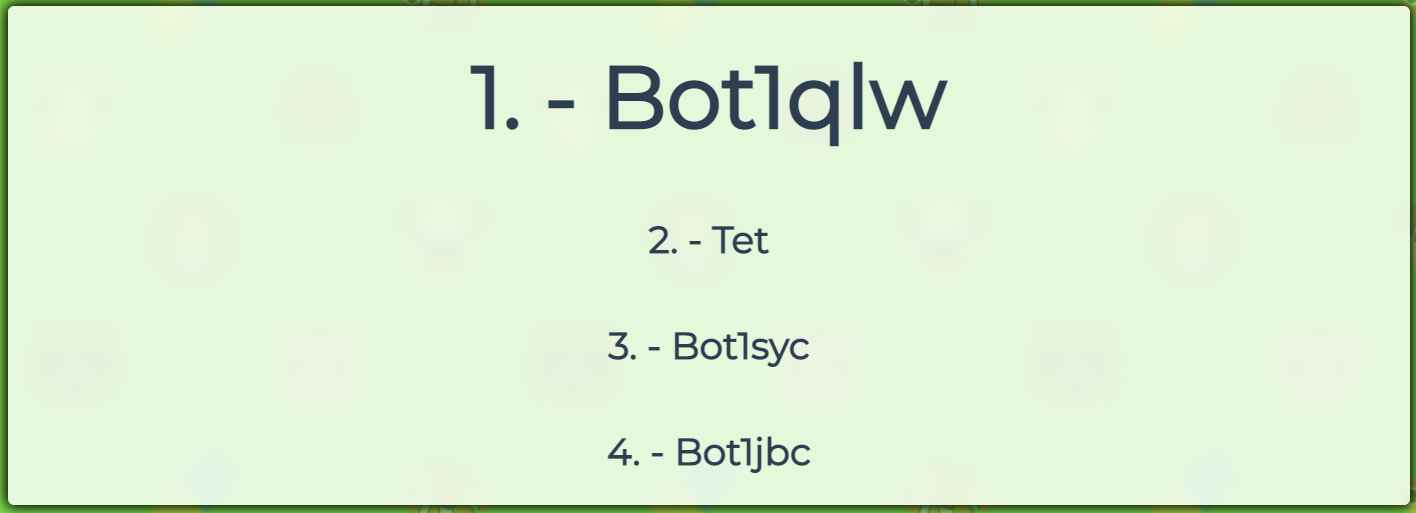
\includegraphics[scale=0.25]{images/ed4cc680904c8608d61522e3b3066dc1.png}
\caption{Eredmények}
\label{fig:ff}
\end{figure}

Miután két játékos is csődöt jelentett, az összes játékosnak egy ranglista jelenik meg  a képernyőjén.